\documentclass[4paper]{article}
\usepackage[spanish]{babel}
%\usepackage[ansinew]{inputenc}
\usepackage[utf8x]{inputenc}
%\usepackage[utf-8]{inputenc}
%\usepackage[T1]{fontenc}
\usepackage{graphicx}
\usepackage{multicol}
\usepackage{float}
%\usepackage{longtable}
%\usepackage{array}
%\usepackage{multirow}
%\usepackage[latin1]{inputenc}
%\inputencoding{latin}
\newcommand{\J}{JavaScript}
\newcommand{\N}{node.js}
\newcommand{\HT}{HTTP}

%\newcommand{\j}{JavaScript }

\renewcommand{\tablename}{Tabla}
\renewcommand{\S}{Introducción a \N}
\author{Manuel Molino Milla}
\title{\textbf{\HT}}
\date{\today}

\begin{document}
\maketitle 
\tableofcontents
\newpage

\section{Introducción}
\subsection{¿Qué es \HT}
\begin{itemize}
\item Es acrónimo de \emph{Hypertext Transfer Protocol}.
\item Es un protocolo de comunicación que permite las transferencias de información en la World Wide Web
\item Fue desarrollado por el \emph{World Wide Web Consortium} y la \emph{Internet Engineering Task Force}
\item  HTTP es un protocolo sin estado, es decir, no guarda ninguna información sobre conexiones anteriores. 
\item El desarrollo de aplicaciones web necesita frecuentemente mantener estado, para esto se usan las cookies, que es información que un servidor puede almacenar en el sistema cliente. 
\item Esto le permite a las aplicaciones web instituir la noción de "sesión", y también permite rastrear usuarios ya que las cookies pueden guardarse en el cliente por tiempo indeterminado.
\end{itemize}
\subsection{Versiones \HT}
\begin{description}
\item[0.9 (lanzada en 1991)] Obsoleta. Soporta sólo un comando, GET, y además no especifica el número de versión HTTP. No soporta cabeceras. Como esta versión no soporta POST, el cliente no puede enviarle mucha información al servidor.
\item[HTTP/1.0 (mayo de 1996)] Esta es la primera revisión del protocolo que especifica su versión en las comunicaciones, y todavía se usa ampliamente, sobre todo en servidores proxy. Permite los métodos de petición GET, HEAD y POST.
\item[HTTP/1.1 (junio de 1999)] Versión más usada actualmente; Las conexiones persistentes están activadas por defecto y funcionan bien con los proxies. También permite al cliente enviar múltiples peticiones a la vez por la misma conexión (pipelining)
\item[HTTP/1.2] Ha quedado como experimental.
\item[HTTP/2 (mayo de 2015)] Esta nueva versión no modifica la semántica de aplicación de http (todos los conceptos básicos continúan sin cambios). Sus mejoras se enfocan en como se empaquetan los datos y en el transporte.
\end{description}

\subsection{Descripción de \HT}
\begin{itemize}
\item Es un protocolo orientado a transacciones y sigue el esquema petición-respuesta entre un cliente y un servidor.
\item   El cliente (se le suele llamar \emph{user agent}) realiza una petición enviando un mensaje,
\item El servidor (se le suele llamar un servidor web) le envía un mensaje de respuesta
\item Ejemplos de cliente son los navegadores web y los spider.
\item Los mensajes HTTP son en texto plano lo que lo hace más legible y fácil de depurar.
\end{itemize}

\subsection{Petciones \HT}
Ejemplo de petición \HT ~ y su correspondiente respuesta:
\begin{verbatim}
usuario@portatil:~$ telnet www.iesvirgendelcarmen.com 80
Trying 2.139.173.60...
Connected to iesvirgendelcarmen.com.
Escape character is '^]'.
GET / HTTP/1.1
Host:www.iesvirgendelcarmen.com

HTTP/1.1 200 OK
Date: Sat, 01 Oct 2016 17:09:46 GMT
Server: Apache/2.4.7 (Ubuntu)
Last-Modified: Fri, 21 Dec 2012 12:13:07 GMT
ETag: "88-4d15bc52d8a2c"
Accept-Ranges: bytes
Content-Length: 136
Vary: Accept-Encoding
Content-Type: text/html

<html>
<head>
<script>
document.location.href="http://www.iesvirgendelcarmen.com/ies/index.php"
</script>
</head>
<body>
</body>
<html>

\end{verbatim}
Ahora la petición la hacemos desde un navegador:
\begin{figure}[H]
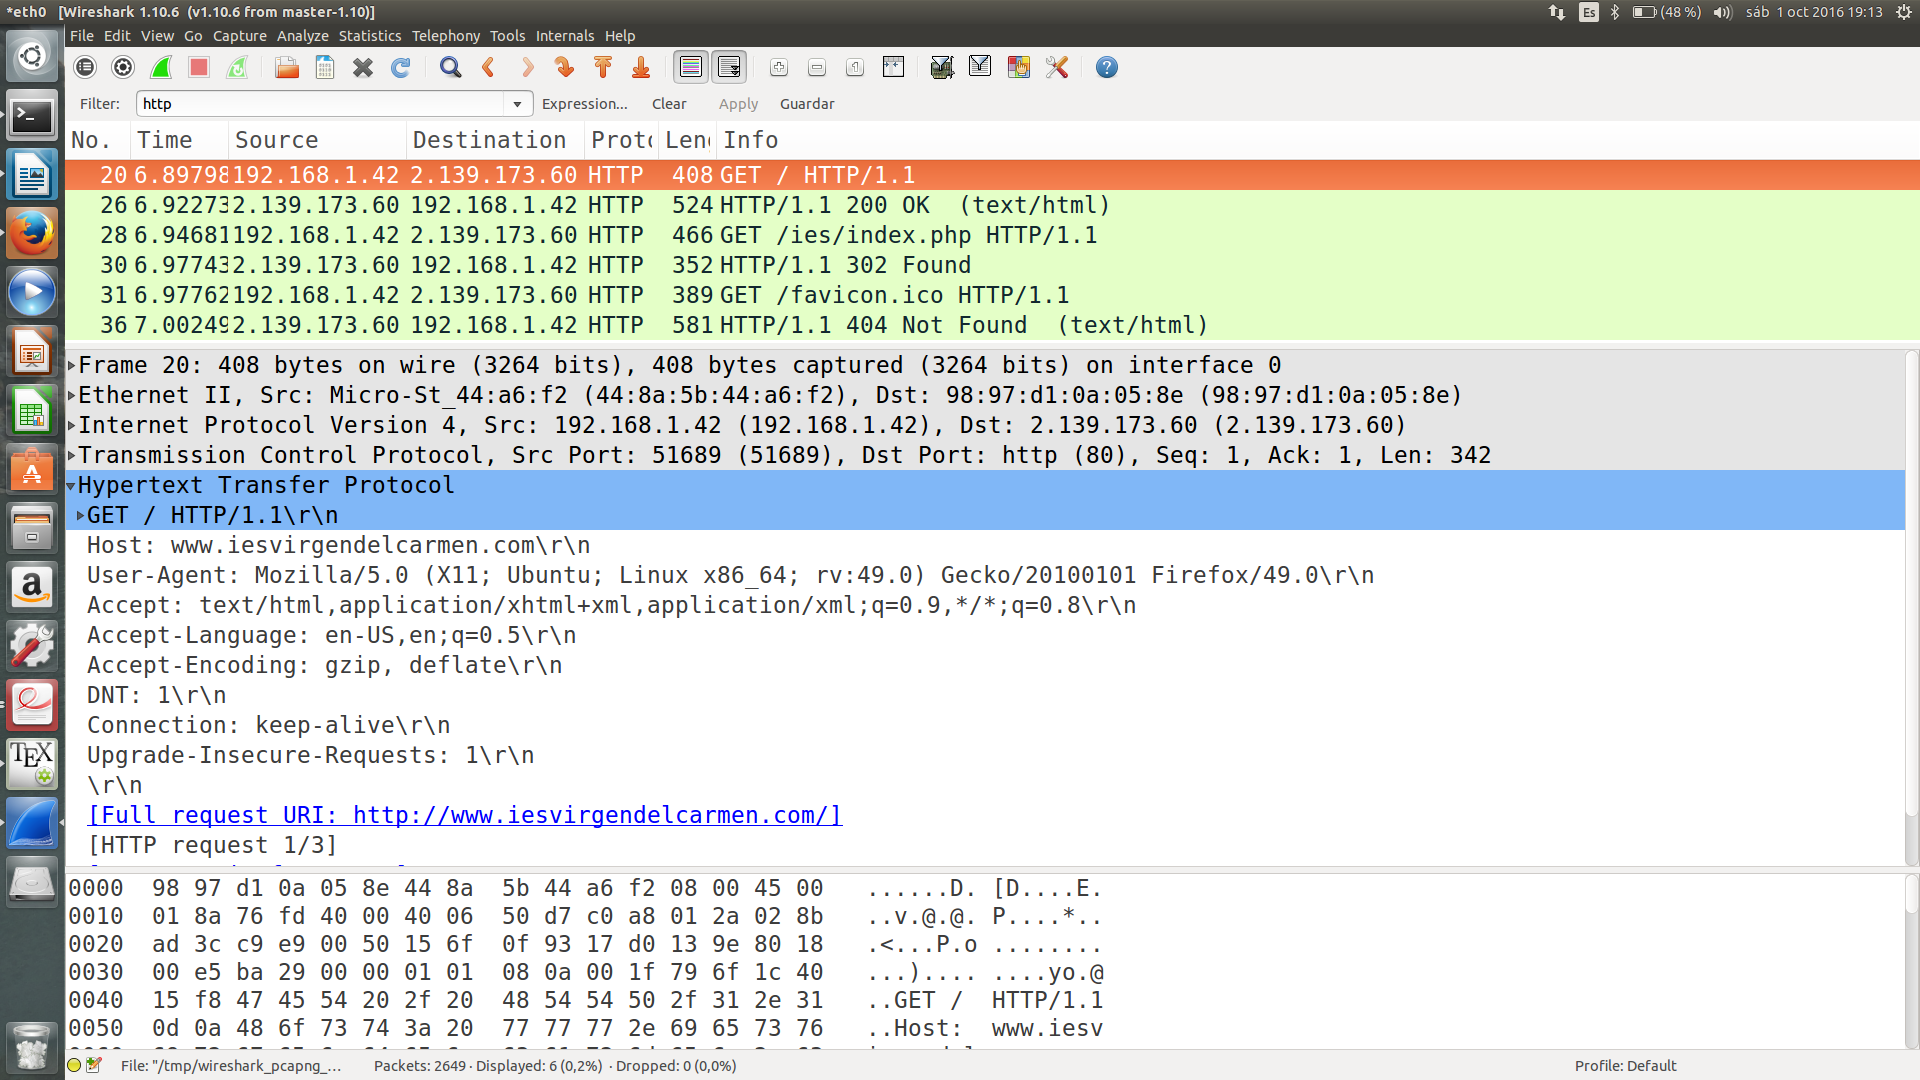
\includegraphics[scale=0.22]{../imagenes/wireshark.png}
\end{figure}

\subsubsection{Métodos de petición \HT}
\begin{itemize}
\item HTTP define una serie predefinida de métodos de petición (algunas veces referido como \emph{verbos}) que pueden utilizarse.
\item El protocolo tiene flexibilidad para ir añadiendo nuevos métodos y para así añadir nuevas funcionalidades. 
\item El número de métodos de petición se han ido aumentando según se avanzaban en las versiones
\item Cada método indica la acción que desea que se efectúe sobre el recurso identificado.
\item Métodos mas comunes:
\begin{description}
\item[HEAD] Se solicita solo la cabecera de respuesta, no el cuerpo.
\item[GET] Solicitamos tanto cabecera como respuesta.
\item[POST] Envía los datos para que sean procesados por el recurso identificado. Los datos se incluirán en el cuerpo de la petición. Ejemplo un formulario.
\item[PUT] Sube, carga o realiza un upload de un recurso especificado.
\item[DELETE] Borra el recurso especificado.
\item[OPTIONS] Indica los métodos soportados por el servidor.
\end{description}
\end{itemize}
Ejemplo de uso del método \emph{OPTIONS}:
\begin{verbatim}
usuario@portatil:~$ telnet www.iesvirgendelcarmen.com 80
Trying 2.139.173.60...
Connected to iesvirgendelcarmen.com.
Escape character is '^]'.
OPTIONS / HTTP/1.1
Host:www.iesvirgendelcarmen.com

HTTP/1.1 200 OK
Date: Sat, 01 Oct 2016 17:48:23 GMT
Server: Apache/2.4.7 (Ubuntu)
Allow: GET,HEAD,POST,OPTIONS
Content-Length: 0
Content-Type: text/html
\end{verbatim}

\subsection{Respuesta \HT}
Las respuestas constan de una \textbf{cabecera} y un \textbf{cuerpo}. En la cabecera nos encontramos datos como:
\begin{itemize}
\item Content-Length (longitud del mensaje)
\item Accept-Encoding (indica el método de compresión aceptado)
\item Accept-Charset (indica el código de caracteres aceptado)
\item Accept (indica el MIME aceptado)
\item Server (indica el tipo de servidor)
\item Location (indica donde está el contenido)
\item Date (fecha de creación)
\item Set-Cookie, Cookie para las cookies.
\item \dots
\end{itemize}
También se encuentran los códigos de respuesta que indica que ha pasado con la petición:
\begin{description}
\item[Códigos con formato 1xx:] Indica que la petición ha sido recibida y se está procesando.
\item[Códigos con formato 2xx:] Respuestas correctas. Indica que la petición ha sido procesada correctamente.
\item[Códigos con formato 3xx:] Respuestas de redirección. Indica que el cliente necesita realizar más acciones para finalizar la petición.
\item[Códigos con formato 4xx:] Errores causados por el cliente. Indica que ha habido un error en el procesado de la petición a causa de que el cliente ha hecho algo mal.
\item[Códigos con formato 5xx:] Errores causados por el servidor. Indica que ha habido un error en el procesado de la petición a causa de un fallo en el servidor.
\end{description}
\begin{figure}[H]
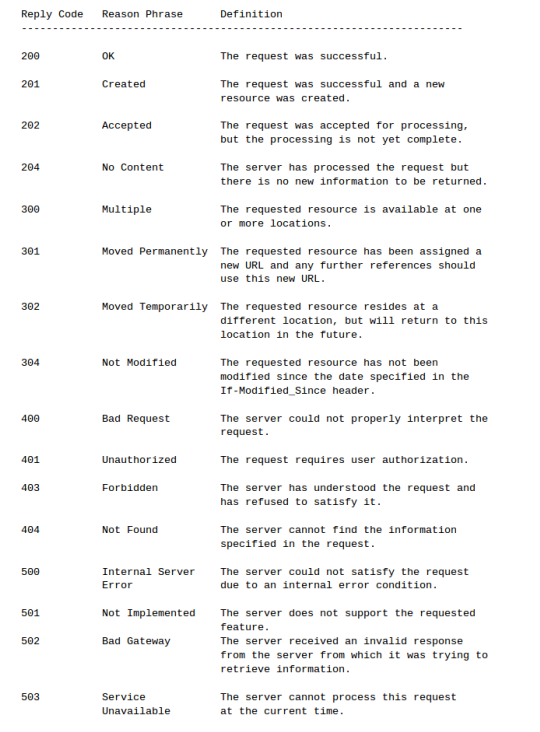
\includegraphics[scale=1]{../imagenes/codigos.png}
\end{figure}
\newpage

\subsection{Protocolos TCP/IP}
\begin{figure}[H]
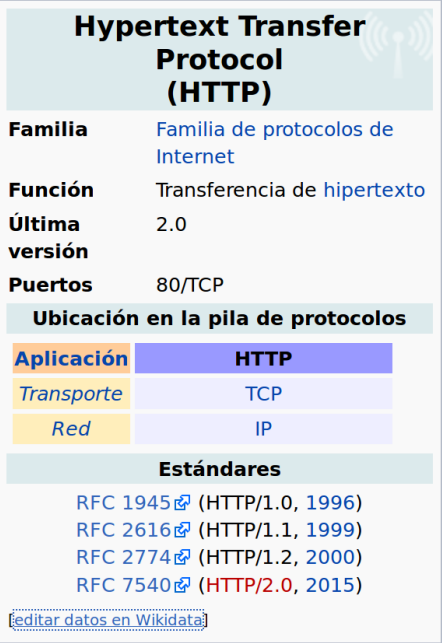
\includegraphics[scale=1.2]{../imagenes/http.png}
\end{figure}
\newpage

\subsection{URI}
\begin{itemize}
\item URI son las siglas en inglés de Uniform Resource Identifier (en español identificador uniforme de recursos),
\item Sirve para identificar recursos en Internet
\item Tene un formato estándar definido
\begin{verbatim}
    esquema://máquina/directorio/archivo#fragmento
\end{verbatim}
\item Ejemplos:
\begin{description}
\item[http] http:\/\/www.pierobon.org/iis/review1.htm
\item[mailto] mailto:someone{@}example.com 
\item[file] file:///home/someuser/somefile.txt
\end{description}
\end{itemize}
En relación a las URL:
\begin{itemize}
\item URL son las siglas en inglés de uniform resource locator (en español, localizador uniforme de recursos)
\item Sirve para nombrar recursos en Internet. 
\item Su propósito es asignar una dirección única a cada uno de los recursos disponibles en Internet, como por ejemplo páginas, imágenes, vídeos, \dots
\item Una URL tiene un formato estándar, que es:
\begin{verbatim}
    esquema://máquina/directorio/archivo
\end{verbatim}
\item El formato específico para HTTP es:
\begin{verbatim}
    http://<máquina>:<puerto>/<path>?<cadena de búsqueda>
\end{verbatim}
\item Se le llama URL semántica a una URL que tiene un formato más fácilmente entendible o interpretable por alguien que la lee. 
\item Ejemplo:
\begin{verbatim}
    URL no semántica: http://ejemplo.com/principal.php?page=noticias
    URL semántica: http://ejemplo.com/noticias
\end{verbatim}
\end{itemize}
El path hace referencia donde se encuentra ubicado el recurso en el servidor web:
\begin{figure}[H]
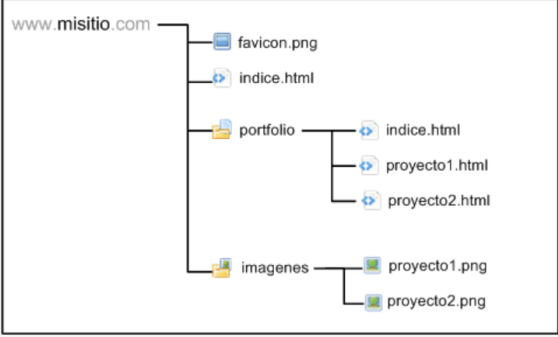
\includegraphics[scale=1]{../imagenes/sitioweb.png}
\end{figure}
La URL para acceder pueden ser:
\begin{verbatim}
www.sitio.com
www.sitio.com/portafolio
\end{verbatim}
Las direcciones a utilizar pueden ser relativas o absolutas a la hora de especificar los recursos en el sitio web. Ejemplo:
\begin{itemize}
\item / \emph{especifica el sitio}
\item /portafolio \emph{especifica la ubicación del recurso de forma absoluta}
\item portafolio \emph{especifica la ubicación del recurso de forma relativa}
\item /imagenes/proyecto1.png \emph{absoluta}
\item imagenes/proyecto1.png \emph{relativa}
\end{itemize}

%\subsection{Ejercicio}
%\begin{itemize}
%\item Instala un servidor web en tu equipo y crea una estructura de sitio web del proyecto anterior. Comprueba su funcionamiento. Los documentos del proyectos están en la plataforma.
%\item Crea un nuevo proyecto en tu sitio web que incluya un fichero \emph{index.html} que incluya un formulario con tres campos: nombre, apellidos y dni/nif. Valida el dni o nif usando un script de javascript que se encuetre en una carpeta denominada \emph{script}
%\item Crea un fichero denominado telefono.html que solicite un número de teléfono y realiza una validación con \emph{HTML5}. Un número de teléfono es válido si y solo si, empieza por 6, 7, 8 o 9 y tiene 9 dígitos. 
%\end{itemize}

\subsection{Creando servidor web con node}
\begin{verbatim}
var http = require("http");
var server = http.createServer(function(request, response) {
  response.writeHead(200, {"Content-Type": "text/html"});
  response.write("<!DOCTYPE 'html'>");
  response.write("<html>");
  response.write("<head>");
  response.write("<title>Hello World Page</title>");
  response.write("</head>");
  response.write("<body>");
  response.write("Hello World!");
  response.write("</body>");
  response.write("</html>");
  response.end();
});

server.listen(4000);
console.log("Server is listening");
\end{verbatim}

\begin{itemize}
\item La primera línea carga el módulo \emph{\HT}
\item \emph{http} es un objeto que tiene el método \emph{createServer} que usa como argumentos una \emph{callback} que incluye la petición (\emph{request}) y la respuesta \emph{\emph{response}}. El uso de la \emph{callback} es crear un servicio \textbf{no bloqueante y asíncrono acorde con la filosofía de nodejs.}
\item Tanto \emph{request} como \emph{response} son objetos, por lo que disponemos de métodos para tratar la petición y la respuesta.
\item En el caso de la respuesta se ha usado el método \emph{writeHead} para especificar la respuesta, en este caso el código de estado y el tipo de respuesta. Aunque por defecto hay otras características incluidas en la respuesta.
\item Y otro método \emph{write} para especificar el cuerpo de la respuesta. Se usa una codificación UTF-8 por defecto.
\item Y por último el método \emph{end} para indicar la finalicación de la respuesta.
\item Luego tenemos el método \emph{listen} que especifica el puerto.
\end{itemize}
\subsubsection{Sirviendo páginas estática}
Si incluimos como primera línea tras el callback que gestiona las peticiones web, la siguiente sentencia:
\begin{verse}
console.log(request.url);
\end{verse}
Nos mostrará el \emph{path} de la petición y partir de aquí podemos decidir que contenido servir.\\
Ya podemos servir contenido estático del sitio. Supongamos la estructura de un sitio web como pueda ser:
\begin{figure}[H]
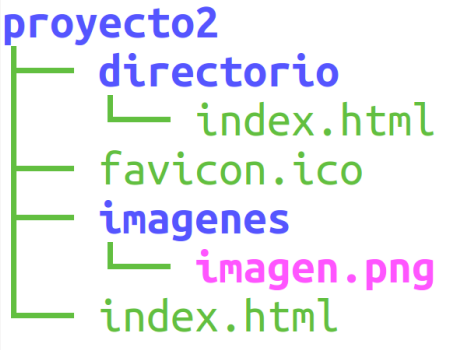
\includegraphics[scale=1]{../imagenes/proyecto.png}
\end{figure}
\newpage
Un servidor que atienda a dichas peticiones podría ser:
\begin{verbatim}
var fs = require('fs');
var http = require("http");
var path = require('path');
__dirname+='/proyecto2/'; //establecemos el directorio de trabajo
var server = http.createServer(function(request, response) {
    //petición de la página índice
    if (request.url === '/' || request.url === '/index.html'){
      fs.readFile(__dirname+'/index.html',function(err,data){
        if (err) throw err;
        response.write(data);
        response.end();
      });
    }
    //petición del favicon.ico
    else if (request.url === '/favicon.ico' || request.url === '/index.html'){
      fs.readFile(__dirname+'/favicon.ico',function(err,data){
        if (err) throw err;
        response.write(data);
        response.end();
      });
    }
    //petición para la página índice de la carpeta directorio
    else if (request.url === '/directorio/' || request.url === '/directorio/index.html'){
      fs.readFile(__dirname+'/directorio/index.html',function(err,data){
       if (err) throw err;
       response.write(data);
       response.end();
      });
    }
    //dejamos para el final las imágenes
    else {
      var patron = /imagenes\/\w+.png$/;
      if (patron.test(request.url)){
      var imagenes = request.url.split('/');
      fs.readFile(__dirname+'/imagenes/'+imagenes[2],function(err,data){
       if (err) throw err;
       response.write(data);
       response.end();
      });
    }
    }
});
server.listen(4000);
console.log("Server is listening");
\end{verbatim}
\subsection{Ejercicio}
Crea un servidor web que atienda las siguientes peticiones:
\begin{itemize}
\item Para la url principal muestre todos los datos de la base de datos de mongo, puedes usar como módulos \emph{mongodb} o \emph{mongoose}
\item Hay que modularizar la aplicación, puedes usar las funciones de acceso a la base de datos anterior.
\end{itemize}
\end{document}
